% !TEX encoding = UTF-8
% !TEX TS-program = pdflatex
% !TEX root = ../Lahmer_Abdelilah_tesi.tex
% !TEX spellcheck = it-IT

%**************************************************************
\chapter{Il progetto di Stage}

\section{Pianificazione del lavoro}
%In questo inizio di sezione parlerò della pianificazione del lavoro per il progetto di stage in fatto di tempistiche.
Per raggiungere gli obiettivi pianificati nel piano di stage e rispettare i requisiti minimi imposti dall'Università, io e il tutor aziendale abbiamo previsto 304 ore di lavoro, distribuite in circa 8 settimane da 40 ore ciascuna. Ho iniziato lo stage il 17 Maggio 2017 e terminato il 10 Luglio 2017, rimanendo in linea con quanto pianificato inizialmente, senza incorrere in particolari differimenti da quanto programmato.

\subsection{Definizione del piano di lavoro}
%In questa sottosezione parlerò della pianificazione del lavoro per il progetto di stage riportando i dati dal piano di lavoro con la programmazione delle ore da dedicare a ciascuna attività.
	Nei giorni immediatamente precedenti l'inizio dello stage mi sono recato in sede Sopra Steria e ho redatto il Piano di Lavoro, con conseguente revisione del tutor aziendale. In questo documento ho definito gli obiettivi e la pianificazione delle attività, assegnando ad ognuna una tempistica in ore e suddividendo l'intero percorso di stage in tre fasi. Ho specificato inoltre le modalità di interazione col tutor e una previsione delle competenze che sarei andato ad acquisire.\\

Tramite il Piano di Lavoro e la pianificazione dettagliata in esso avrei potuto infatti verificare l'effettivo allineamento tra il lavoro svolto e il lavoro pianificato man mano che il percorso di stage volgeva al termine.\\
	
Settimanalmente inoltre aggiornavo il mio tutor interno sulla mia situazione in relazione alla pianificazione, riportando eventuali scostamenti dal Piano di Lavoro. \\

\newpage

	Le fasi individuate in tale documento sono state:
	
	\begin{itemize}
		\item \textbf{FASE 1 - Formazione tecnica}: durante questa prima fase del percorso formativo era prevista l'introduzione alle modalità di approccio alla programmazione tramite dei corsi a seconda dell'ambiente di sviluppo, tecnologie e linguaggi di programmazione da utilizzare; in particolare era previsto: 
			\begin{itemize}
				\item lo studio e utilizzo dell'ambiente di sviluppo mainframe;
				\item lo studio dei concetti fondamentali del linguaggio di programmazione COBOL\glossario;
				\item lo studio delle modalità di interazione con database DB2;
				\item lo sviluppo di semplici programmi nell'ambito dell'applicazione realizzata da Sopra Steria.
			\end{itemize}
		\item \textbf{FASE 2 - Formazione funzionale}: durante questa seconda fase del percorso formativo era prevista l'introduzione alla metodologia di operatività in ambito funzionale, iniziando a lavorare a stretto contatto con il resto del team della \textit{Business Unit} addetta ai Servizi Finanziari. Erano previste infatti attività di formazione di carattere funzionale in ambito bancario, apprendendo la modalità di collegamento tra quella che è la parte funzionale del sistema con la parte tecnica, introdotta nella FASE 1; in particolare era previsto: 
			\begin{itemize}
				\item lo studio e utilizzo del sistema sviluppato dall'azienda, ovvero ELISE\glossario;
				\item lo studio e utilizzo della parte relativa alla funzionalità di “finanziamenti in Pool\footnote{I finanziamenti in Pool in ambito bancario rappresentano quelli che vengono denominati anche \textit{prestiti sindacati}, sono erogati da un insieme di banche a favore di un'impresa. Scopo di tale raggruppamento è la ripartizione del rischio e dello sforzo di finanziamento.}” all'interno di ELISE;
				\item lo studio delle modalità di trasformazione dei concetti funzionali in tecnici.
			\end{itemize}
		
		\item \textbf{FASE 3 - Analisi tecnica e funzionale modulo “Pool”}: In questa ultima e terza fase del percorso formativo era previsto lo studio della parte tecnica e funzionale di uno dei moduli dell'applicazione orientata ai finanziamenti realizzata da Sopra Steria, ovvero il modulo “Pool”. Era previsto inoltre lo sviluppo in linguaggio COBOL di quelle che sarebbero state le funzionalità studiate ed analizzate nel documento funzionale e tecnico.% In particolare in questa fase del percorso di stage erano previsti:
%			\begin{itemize}
%				\item lo studio e l'analisi del modulo;
%				\item la progettazione dell'analisi funzionale;
%				\item la redazione dell'analisi Funzionale e Tecnica del modulo.
%			\end{itemize}

	\end{itemize}
\leavevmode	\newline

%\newpage
		\begin{center}
		  \bgroup
		  \def\arraystretch{1.4}
		   \setlength\arrayrulewidth{0.6pt}
		   \begin{longtable}{ | p{2.61cm} | p{9cm} |} \hline
		   %\begin{longtable}{ | p{2.5cm} | p{0.5cm} | p{9cm} |} \hline
		   
		    %\cellcolor[gray]{0.9} \textbf{Durata in ore} & \cellcolor[gray]{0.9} & \cellcolor[gray]{0.9} \textbf{Descrizione dell'attività} \\ \hline
		    
		    \cellcolor[gray]{0.9} \textbf{Durata in ore} &  \cellcolor[gray]{0.9} \textbf{Descrizione dell'attività} \\ \hline


			76 	& FASE 1: FORMAZIONE TECNICA \\ \hline

			\tab \tab 24 & Formazione ambiente di sviluppo Mainframe\\
			\cline{2-2}		%\cline{2-2}
			\tab \tab 52 & Formazione linguaggio di programmazione COBOL \\	\hline
			
			76 	& FASE 2: FORMAZIONE FUNZIONALE \\ \hline

			\tab \tab 12 &  Formazione sul sistema sviluppato dall'azienda\\
			\cline{2-2}		%\cline{2-2}
			\tab \tab 12 &   Formazione sulla parte relativa al concetto di “Pool”\\
			\cline{2-2}		%\cline{2-2}
			\tab \tab 52 &  Formazione sulla modalità di trasformazione dei concetti funzionali in tecnici\\	\hline			
			
			152 & FASE 3: ANALISI TECNICA E FUNZIONALE MODULO “POOL” \\ \hline

			\tab \tab 40 &  Analisi modulo \\
			\cline{2-2}		%\cline{2-2}
			\tab \tab 40 &  Progettazione dell'analisi funzionale \\
			\cline{2-2}		%\cline{2-2}
			\tab \tab 72 &   Redazione analisi Funzionale e Tecnica modulo \\	\hline
			
			\caption{Pianificazione delle attività di stage}
			
		    \end{longtable}
		  \egroup
		\end{center}
	
\subsection{Livello di autonomia}
%In questa sottosezione parlerò del livello di autonomia con cui ho svolto lo stage.

	Inizialmente con l'inizio dello stage l'idea era quella di lavorare in un ambiente che mi teneva a stretto contatto con il tutor aziendale, in modo tale da favorire l'interazione e garantire il raggiungimento degli obiettivi prefissati, come da Piano di Lavoro; successivamente però ho scoperto che non sarebbe stato così. Il tutor aziendale infatti, essendo manager di prossimità della sede e facente parte del team degli Analisti Funzionali, era generalmente in trasferte lavorative in sedi distaccate di Sopra Steria oppure dal cliente.\\
	
	Sono stato quindi affiancato da più colleghi della sede per le diverse competenze che dovevo apprendere.\\
	
	Questo tipo di approccio però non è stato positivo; i colleghi a cui sono stato affiancato infatti, soprattutto lato tecnico non sono stati in grado di farmi seguire un percorso di apprendimento proficuo, non avendo particolari metodi di insegnamento oltre ad una visione incompleta dell'architettura dell'applicazione.\\
	
	Questo fattore è stato un deficit rilevante al fine del raggiungimento degli obiettivi prefissati.\\

	Il livello di autonomia che ho raggiunto alla fine del percorso infatti non era sufficiente da poter portare a termine un'attività di sviluppo o analisi in completa indipendenza, necessitavo infatti di saltuarie delucidazioni.\\
	
	La difficoltà di lavoro in modalità autonoma è secondariamente dovuta al fatto che l'ambiente di sviluppo mainframe era a me sconosciuto prima di iniziare l'esperienza di stage, durante il percorso di studi infatti non è mai stato possibile trattare praticamente questo tipo di contesto. La mancanza di basi di natura economica inoltre hanno sfavorito parzialmente l'autonomia sotto l'aspetto funzionale.

\section{Formazione}
%In questo inizio di sezione farò una panoramica sulla formazione che ho ricevuto, sia quella in ambito teorico-economico sia quella in ambito tecnico.

Le prime due fasi del percorso di stage le ho dedicate alla formazione in due ambiti, quello tecnico e quello funzionale. La formazione tecnica si poneva come obiettivo fornire una sufficiente base sul linguaggio di programmazione COBOL e le modalità di sviluppo, utilizzando quest'ultimo, in ambiente mainframe. La formazione funzionale, invece, si poneva come obiettivo quello di apprendimento d'uso di ELISE e dei concetti economici fondamentali utilizzati in esso.

\subsection{Conoscenze economiche acquisite}
%In questa sottosezione parlerò più approfonditamente della formazione in ambito teorico-economico che ho ricevuto e riporterò i macro argomenti trattati, magari con qualche accenno a qualche concetto fondamentale.

Come ho indicato nella sezione dedicata [\ref{ELISE: Extended Loans Integrated System}], ELISE è un complesso sistema di gestione di finanziamenti, esso infatti fornisce un ambiente completo che permette il tracciamento di un prestito da quando questo viene istanziato alla sua estinzione. I concetti di natura teorica indispensabili al concepimento degli stati in cui questo può trovarsi e delle funzionalità predisposte dall'applicazione su di esso sono stati oggetto della formazione teorica ricevuta.\\

Di seguito riporterò le più rilevanti nozioni acquisite.

\paragraph{Finanziamento}
Un finanziamento è un rapporto che intercorre tra almeno due soggetti e consiste nella cessione di una somma di denaro con il vincolo della restituzione di capitali di pari valore o maggiori.\\
Gli elementi costitutivi di un finanziamento sono:
	\begin{itemize}
		\item capitale finanziato;
		\item tasso annuo nominale d'interesse (TAN);
		\item tasso annuo effettivo globale (TAEG);
		\item durata del finanziamento;
		\item l'importo, ed eventuali rate e condizioni.	
	\end{itemize}

L'assegnazione di un prestito avviene dopo una serie di controlli preliminari che il mediatore esegue in base alla situazione economica e professionale del soggetto richiedente, esami che gli permettono di valutare la sicurezza evitando sconvenienti situazioni di insolvenza.\footnote{Wikipedia - Prestito (finanza). URL: \url{https://goo.gl/mwp69N}}

\paragraph{Fido}
Un fido bancario, o affidamento, è definito come l'impegno assunto da una banca a mettere una somma a disposizione del cliente, o di assumere per suo conto un'obbligazione nei confronti di un terzo. Un fido bancario può essere concesso sia ad un privato sia ad un'azienda, tuttavia è quest'ultima la categoria che ricorre maggiormente al credito bancario. Gli affidamenti bancari vengono concessi dagli istituti di credito a seguito di una complessa istruttoria che di norma ha ad oggetto sia i profili reddituali che quelli patrimoniali del soggetto richiedente al fine di stabilire la capacità di restituzione del credito concesso (profilo reddituale) e la solidità finanziaria (profilo patrimoniale).\footnote{Wikipedia - Fido bancario. URL: \url{https://goo.gl/49Wwbs}}

\paragraph{Tasso}
In economia, il tasso di interesse effettivo rappresenta la percentuale dell'interesse su un prestito e l'importo della remunerazione spettante al prestatore. Viene espresso come una percentuale per un dato periodo di tempo e indica quanta parte della somma prestata debba essere corrisposta come interesse al termine del tempo considerato o, da un altro punto di vista, indica il costo del denaro. Il debitore, infatti, ricevendo una somma di denaro, si impegna a pagare una somma superiore a quella ricevuta. La differenza costituisce l'interesse, che viene solitamente calcolato in percentuale sulla somma prestata. Tale percentuale costituisce il tasso di interesse. Il tasso d'interesse è variabile anche in funzione della moneta di riferimento, del rischio connesso alla solvibilità del debitore e della lunghezza del periodo di riferimento.\footnote{Wikipedia - Tasso d'interesse. URL: \url{https://goo.gl/AHpfia}}

\paragraph{Piano di ammortamento}
Il piano di ammortamento è un programma di estinzione di debito o di abbassamento o estinzione del capitale di credito. Esistono diversi tipi di piano di ammortamento:
	\begin{itemize}
		\item Ammortamento a rate costanti (francese);
		\item Ammortamento con quote capitali costanti (italiano).	
	\end{itemize}
Il piano utilizzato nel sistema bancario italiano è quello alla francese, cioè a rate costanti. Visualizzando il piano di ammortamento ci si accorge che:
	\begin{itemize}
		\item la rata è sempre la stessa (sempre che il tasso non cambi);
		\item la quota interessi è pari al tasso di interesse del periodo per il debito residuo alla fine del periodo precedente;
		\item la quota capitale è la differenza tra rata e quota interessi.\footnote{Wikipedia - Piano di ammortamento. URL: \url{https://goo.gl/vtBdix}}
	\end{itemize}

\paragraph{Finanziamento in Pool}
I prestiti sindacati, conosciuti anche come "finanziamenti in pool", sono erogati da un consorzio di banche (il pool) a favore di un'impresa. Scopo di tale raggruppamento è la ripartizione del rischio e dello sforzo di finanziamento; il pool si scioglie una volta ultimata l'operazione. I prestiti in pool fanno parte di quella categoria di finanziamenti a medio-lungo termine che concedono le banche. I prestiti in pool fanno parte di quella categoria di finanziamenti a medio-lungo termine che concedono le banche. All'interno di un pool si distingue solitamente:
	\begin{itemize}
		\item la banca \textit{arranger} che si assume l'onere dell'organizzazione (in ELISE questa si chiama banca "\textit{rappresentante}");
		\item la banca capofila, (spesso coincide con la banca \textit{arranger}) che coordina la sindacazione;
		\item la banca agente che cura tutti gli aspetti amministrativi dopo l'operatività del prestito;
		\item la banca partecipante che eroga una quota parte del prestito.\footnote{Wikipedia - Prestiti sindacati. URL: \url{https://goo.gl/nQyvFh}}
	\end{itemize}

\subsubsection{ELISE}
\label{ELISE}
%In questa sotto sottosezione descriverò ELISE e spiegherò i suoi scopi e funzionalità principali, collegando infine il tutto con le attività formazione teorico-economiche che ho applicato in essa dopo averle acquisite.

Nella formazione sotto l'aspetto funzionale uno dei principali obiettivi era anche quello di apprendere la modalità d'uso di ELISE, ovvero l'applicazione ambito di progetto aziendale. Durante questa fase di formazione ho cercato di acquisire capacità di navigazione all'interno di essa. Quest'attività di apprendimento è strettamente legata alla formazione sui concetti teorico-economici discussi nella sezione precedente.\\

Nel formarmi su questo complesso sistema ho afferrato un concetto molto importante: ELISE è un applicazione orientata ai "\textit{Prodotti di Finanziamento}", ogni prestito istanziabile infatti fa parte di un prodotto, che è visto come una tipologia di finanziamento offerto dall'istituto di credito. Ogni prodotto ha le proprie condizioni, che possono essere derogabili o meno. Tali condizioni possono variare nel tempo, per questo nel processo di richiesta di un finanziamento il prodotto viene clonato, assieme alle rispettive condizioni, al fine di salvare la versione utilizzata.\\

Le funzionalità principali di ELISE oggetto di formazione sono state:
	\begin{itemize}
	\item creazione dei vari tipi di finanziamento;
	\item pagamento rate di un dato finanziamento;
	\item estinzione di un dato finanziamento;
	\item modifica delle condizioni dei vari "Prodotti di Finanziamento";
	\item creazione di pool;
	\item creazione di finanziamenti in pool;
	\item stipula di contratti di finanziamento.
	\end{itemize}

\subsection{Tecnologie utilizzate}
%In questa sottosezione parlerò più dettagliatamente delle tecnologie che ho utilizzato.

\subsubsection{Piattaforma host}
%In questa sotto sottosezione introdurrò la piattaforma host su cui ho lavorato, spiegando nel dettaglio la struttura della rete e i vari elaboratori su cui il codice viene immagazzinato ed eseguito.

Nel formarmi sotto l'aspetto tecnico, ovvero sulle metodologie di programmazione \textit{back-end}\glossario, ho avuto modo di comprendere e avere un'idea di quella che è l'architettura della piattaforma \textit{host}.\\

Tale architettura si sviluppa su più sedi, che comprendono le diverse filiali dell'istituto di credito, assieme a quelle delle aziende di ICT\glossario\ addette alla manutenzione dei sistemi informativi della banca e dell'implementazione all'interno di essi di nuove funzionalità, com'è il caso di Sopra Steria.\\

Gli elaboratori principali, ovvero i mainframe, sono localizzati all'interno delle unità CED\glossario\ degli istituti finanziari, il colloquio con questi avviene tramite transazioni CICS\glossario\footnote{Transazioni CICS. URL: \url{https://goo.gl/QKRXTe}}, anche dagli uffici centrali delle banche che generalmente coincidono con la sede in cui questi sono installati.\\

Per lo sviluppo su questo tipo di piattaforma è necessario l'uso degli strumenti, quali emulatori e ambienti di sviluppo, illustrati nella sezione relativa alle tecnologie e strumenti a supporto di processi e servizi [\ref{Ambienti di sviluppo ed emulatori}].\\

Nel processo di rilascio di nuove funzionalità il team di sviluppatori segue un procedimento di \textit{packaging} dei sorgenti a cui sono state apportate modifiche, al fine di "\textit{portare in produzione}", in gergo, le nuove implementazioni.\\

Questo procedimento installa sull'elaboratore centrale il nuovo applicativo, effettuando un trasferimento fisico sulla macchina.\\

Di seguito riporto una raffigurazione indicativa dell'architettura su cui si basa il progetto ELISE:

	\begin{figure}[H]
		\centering
	   	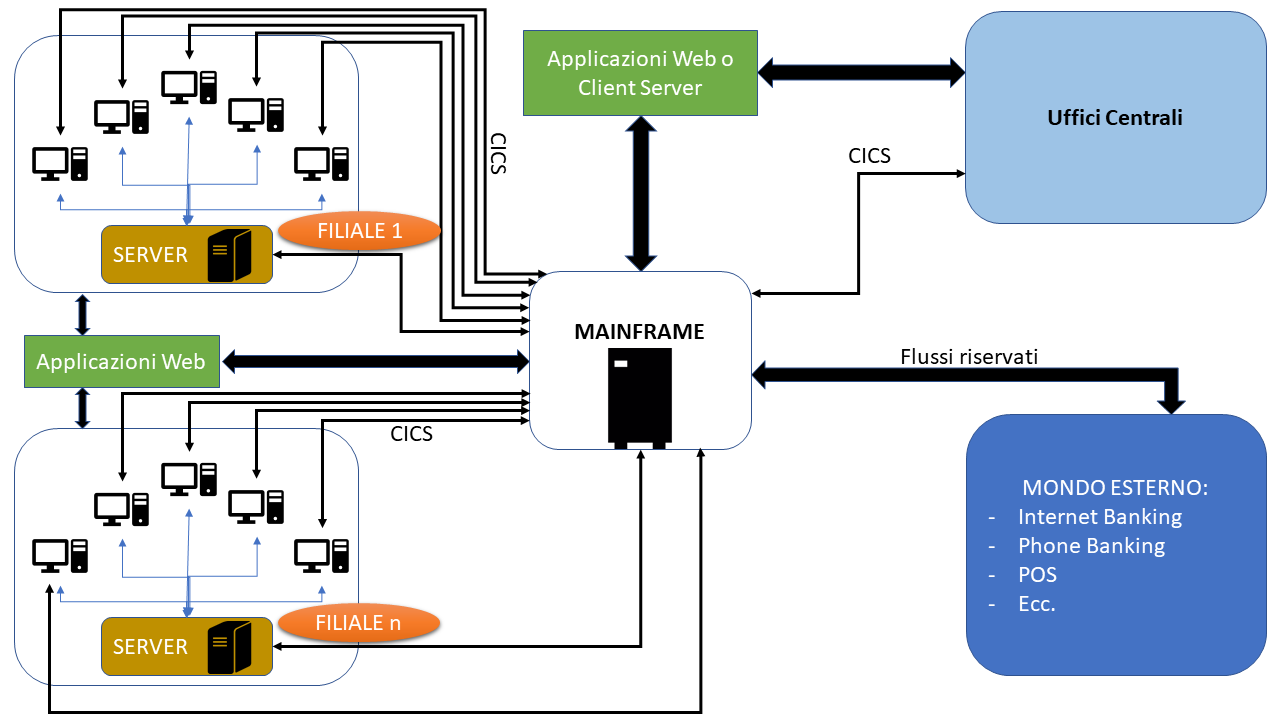
\includegraphics[width=1\textwidth]{immagini/Architettura}
	   	\caption{Architettura piattaforma Host - Fonte schema:\\ \tab \url{https://goo.gl/gZFJRF} }
	\end{figure}

	
\subsubsection{COBOL}
%In questa sotto sottosezione riporterò i concetti fondamentali di quello che è il linguaggio di programmazione COBOL e l'uso che se ne fa, riportando poi alcuni esempio dei formalismi principali tramite i quali i moduli delle applicazioni host elaborano i dati.

Durante la formazione sulla parte tecnica gran parte del tempo lo ho dedicato al linguaggio COBOL.\\

In un programma scritto in linguaggio COBOL è indispensabile, secondo la prassi aziendale, la presenza delle seguenti divisioni:
\begin{itemize}

\item \textbf{IDENTIFICATION DIVISION}: in questa divisione vengono incluse informazioni generiche come il nome del programma, la data di creazione e la funzione del programma;

\item \textbf{ENVIRONMENT DIVISION}: in questa divisione viene indicato l'ambiente in cui viene utilizzato il programma (il tipo di macchina), l'eventuale presenza di file di input-output e la modalità di controllo di questi ultimi;

\item \textbf{DATA DIVISION}: in questa divisione vengono definite le aree di variabili e costanti utilizzate all'interno del programma;

\item \textbf{LINKAGE SECTION}: in questa sezione, facente parte della DATA DIVISION, vengono definite le aree di comunicazione comuni ai moduli di ELISE, assieme alle interfacce utilizzate all'interno del programma;

\item \textbf{PROCEDURE DIVISION}: in questa divisione è definito il corpo elaborativo del programma, all'interno di questo \textit{scope} infatti viene specificato il flusso del modulo.
\end{itemize}

Di seguito riporto un frammento di codice con la struttura ideale di un programma scritto in linguaggio COBOL:

\begin{lstlisting}[language=cobol, caption={Struttura ideale di un programma COBOL}]
ABDELI IDENTIFICATION DIVISION.
ABDELI PROGRAM-ID.   ESCOBOL.
ABDELI AUTHOR.       ABDELILAH LAHMER.
ABDELI DATE-WRITTEN. 2017-12-01.
ABDELI*
ABDELI ENVIRONMENT DIVISION.
ABDELI*
ABDELI DATA DIVISION.
ABDELI*
ABDELI WORKING-STORAGE SECTION.                         
ABDELI*
ABDELI PROCEDURE DIVISION.
ABDELI*-------COMMENTO: INIZIO PROCEDURE DIVISION-------
ABDELI INIZIO-PGM.
ABDELI     DISPLAY 'INIZIO PROGRAMMA ESCOBOL'
ABDELI 	   PERFORM CORPO-PGM
ABDELI     PERFORM STAMPA-FINE
ABDELI .
ABDELI*
ABDELI CORPO-PGM.
ABDELI     DISPLAY 'ESECUZIONE CORPO PROGRAMMA ESCOBOL'.
ABDELI*
ABDELI STAMPA-FINE.
ABDELI     DISPLAY 'FINE PROGRAMMA ESCOBOL'.
ABDELI*--------COMMENTO: FINE PROCEDURE DIVISION--------
\end{lstlisting}

Come si nota dal frammento di codice precedente l'area che verrà interpretata dal compilatore va dalla ottava colonna in poi, le prime sei colonne infatti sono adibite al cosiddetto "\textit{segnalino}" (accennato nella sezione [\ref{Vincoli del progetto}]) e la settima all'eventuale commento della riga.\\

%\leavevmode	\newline

L'uso che se ne fa del COBOL nei sorgenti prodotti è principalmente quello di interfacciamento con il database, interrogandolo in lettura, modifica dei dati a seconda delle funzioni richiamate dall'utente che interagisce con l'interfaccia \textit{web} e scrittura dei dati, in caso la funzione richiamata lo richieda.\\

%\newpage
I principali costrutti indispensabili per l'elaborazione dei dati sono:

\begin{itemize}
	\item \textbf{IF}: permette di condizionare l'esecuzione di un gruppo di istruzioni;
	\begin{lstlisting}[language=cobol, caption={Esempio d'uso costrutto IF in COBOL}]
ABDELI*--------ESEMPIO USO  COSTRUTTO IF--------
ABDELI 	IF DATO-INPUT IS NUMERIC
ABDELI 	  PERFORM ELABORA-NUMERICO
ABDELI	ELSE
ABDELI	  PERFORM ELABORA-ALFANUMERICO
ABDELI	END-IF.
	\end{lstlisting}
	
	\item \textbf{PERFORM}: permette il richiamo di una funzione presente nel programma; consente infatti di eseguire un gruppo di istruzioni contenute all’interno di sezioni o di paragrafi della divisione PROCEDURE DIVISION, riprendendo poi il flusso dall'istruzione successiva;
	\begin{lstlisting}[language=cobol, caption={Esempio d'uso costrutto PERFORM in COBOL}]
ABDELI*------ESEMPIO USO COSTRUTTO PERFORM------
ABDELI FUNZIONE-CHIAMANTE.
ABDELI     DISPLAY 'FUNZIONE-CHIAMANTE'
ABDELI 	   PERFORM CHIAMA-FUN2.
ABDELI     DISPLAY 'FINE FUNZIONE-CHIAMANTE'
ABDELI*
ABDELI CHIAMA-FUN2.
ABDELI     DISPLAY 'ESECUZIONE CORPO CHIAMA-FUN2'.
	\end{lstlisting}

	\item \textbf{EVALUATE}: permette la gestione di più condizioni, specificando il modo di elaborazione di ognuno in caso si verifichi, evitando di utilizzare molteplici costrutti IF innestati;
	\begin{lstlisting}[language=cobol, caption={Esempio d'uso costrutto EVALUATE in COBOL}]
ABDELI*-----ESEMPIO USO  COSTRUTTO EVALUATE-----
ABDELI 	EVALUATE DATO-INPUT
ABDELI	  WHEN 'NUMERICO'
ABDELI 	    PERFORM ELABORA-NUMERICO
ABDELI	  WHEN 'ALFANUMERICO'
ABDELI	    PERFORM ELABORA-ALFANUMERICO
ABDELI	END-EVALUATE.
	\end{lstlisting}

\newpage

	\item \textbf{MOVE}: permette la copia o assegnazione di un valore ad una o più variabili di destinazione;
	\begin{lstlisting}[language=cobol, caption={Esempio d'uso costrutto MOVE in COBOL}]
ABDELI*-------ESEMPIO USO  COSTRUTTO MOVE-------
ABDELI MOVE ZERO		TO VAR-INDICE.
	\end{lstlisting}

%\newpage


	\item \textbf{SET}: in quel che è la prassi aziendale questo costrutto viene utilizzato per settare una variabile booleana;
	\begin{lstlisting}[language=cobol, caption={Esempio d'uso costrutto SET in COBOL}]
ABDELI*--------ESEMPIO USO COSTRUTTO SET--------
ABDELI SET FLAG		TO TRUE.
	\end{lstlisting}

	\item \textbf{VARYING}: permette la gestione di un contatore numerico specificando il valore di inizializzazione dopo il FROM, l'incremento ad ogni ciclo dopo il BY e la condizione di uscita dopo l'UNTIL, in questo modo è possibile utilizzare dei cicli di elaborazione dati in modo semplice.
	\begin{lstlisting}[language=cobol, caption={Esempio d'uso costrutto VARYING in COBOL}]	
ABDELI*------ESEMPIO USO COSTRUTTO VARYING------
ABDELI PERFORM VARYING VAR-INDICE FROM 1 BY 1
ABDELI  UNTIL VAR-INDICE > LUNGHEZZA
ABDELI   DISPLAY 'INDICE: ' VAR-INDICE
ABDELI END-PERFORM
	\end{lstlisting}
		
\end{itemize}
	
\subsubsection{JCL}
%In questa sotto sottosezione riporterò i concetti fondamentali di quello che è il linguaggio di scripting JCL e riportando qualche esempio dell'uso che se ne fa, ovvero il controllo dell'esecuzione di moduli COBOL.
Durante la formazione sulla parte tecnica ho avuto modo di operare superficialmente con il linguaggio JCL\glossario. Come accennato nella sezione relativa ai linguaggi utilizzati [\ref{Linguaggi lato Host}] il JCL è un linguaggio usato con lo scopo di dire all'elaboratore quali programmi eseguire, usando quali file di input e quali generare in output. L'uso che se ne fa in azienda consiste nel programmare e regolare l’esecuzione di programmi in modalità batch\glossario. \\

Per il JCL non è stata prevista formazione, come da Piano di Lavoro; una volta apprese le modalità di sviluppo però ne ho scoperto l'indispensabilità.\\

\newpage

Di seguito riporto un frammento di codice\footnote{JCL - Eseguire programmi COBOL. URL: \url{https://goo.gl/bpaFUC}} in linguaggio JCL che esegue il programma MYCOBB a titolo di esempio:

%\begin{lstlisting}[language=C++]
\begin{lstlisting}[language=Cobol, caption={Struttura ideale di un programma JCL}]
//STEP001  EXEC PGM=IKJEFT01
//*
//STEPLIB  DD DSN=MYDATA.URMI.DBRMLIB,DISP=SHR
//*
//input files
//output files
//SYSPRINT DD SYSOUT=*
//SYSABOUT DD SYSOUT=*
//SYSDBOUT DD SYSOUT=*
//SYSUDUMP DD SYSOUT=*
//DISPLAY  DD SYSOUT=*
//SYSOUT   DD SYSOUT=*
//SYSTSPRT DD SYSOUT=*
//SYSTSIN  DD *
    DSN SYSTEM(SSID)
    RUN PROGRAM(MYCOBB) PLAN(PLANNAME) PARM(param)
    LIB('MYDATA.URMI.LOADLIB')
    END
/*
\end{lstlisting}

\section{Processo di sviluppo}
%In questo inizio di sezione introdurrò la fase di stage relativa al processo di sviluppo del progetto di stage.
%Al termine delle prime fasi di formazione ero portato alla realizzazione di un progetto di stage che consisteva nella redazione di un'Analisi Funzionale e Tecnica del modulo "Pool", assieme all'implementazione di quanto studiato nell'Analisi Funzionale. Una volta entrato nell'ambiente lavorativo ed avuto un'idea di quella che era l'architettura di ELISE sono riuscito a concepire la difficoltà di questi compiti, sopratutto in relazione al tempo di formazione che avevo avuto. Il modulo "Pool" di cui si richiedeva l'analisi, infatti, era pressoché la metà dell'intera architettura del sistema, oltre al fatto di essere già implementato.\\
%
%Visto ciò ho scelto di analizzare un'altra funzionalità, in parte collegata al concetto di Pool, ovvero quella di "calcolo delle Commissioni di Mancato Utilizzo (CMU)"\footnote{La commissione di mancato utilizzo viene calcolata sull'importo non impiegato di un finanziamento, che però è stato predisposto dall'istituto di credito a favore del cliente; generalmente questa commissione ammonta allo 0,50\% su base annua.}, anch'essa già implementata ma solo a scopo di esercitazione mi preparavo ad esaminarla.

\subsection{Analisi dei requisiti}
%In questa sottosezione descriverò l'attività di analisi dei requisiti e riporterò il modo in cui è stata svolta.

Al termine delle prime fasi di formazione ero portato alla realizzazione di un progetto di stage che consisteva nella redazione di un'Analisi Funzionale e Tecnica del modulo "Pool", assieme all'implementazione di quanto studiato nell'Analisi Funzionale. Una volta entrato nell'ambiente lavorativo ed avuto un'idea di quella che era l'architettura di ELISE sono riuscito a concepire la difficoltà di questi compiti, sopratutto in relazione al tempo di formazione che avevo avuto. Il modulo "Pool" di cui si richiedeva l'analisi, infatti, era pressoché la metà dell'intera architettura del sistema, oltre al fatto di essere già implementato.\\

Visto ciò ho scelto di analizzare un'altra funzionalità, in parte collegata al concetto di Pool, ovvero quella di "calcolo delle Commissioni di Mancato Utilizzo (CMU)"\footnote{La commissione di mancato utilizzo viene calcolata sull'importo non impiegato di un finanziamento, che però è stato predisposto dall'istituto di credito a favore del cliente; generalmente questa commissione ammonta allo 0,50\% su base annua.}, anch'essa già implementata ma solo a scopo di esercitazione mi preparavo ad esaminarla.\\

	Come prima attività nel processo di sviluppo di nuove funzionalità l'azienda esegue delle attività di consulenza assieme al cliente, sottoscrivendo infine i contratti una volta giunti ad un accordo sui requisiti da soddisfare.\\
	
	Questa fase di raccolta dei requisiti ha un'importanza essenziale al fine di fornire un prodotto che rispetti le aspettative del cliente, questa attività infatti richiede di analizzare con cura i loro bisogni, cercando di capire quali soluzioni possano soddisfarli al meglio. Effettuare una buona analisi in questa fase garantisce che le successive attività di progettazione e codifica avvengano su una base solida, senza il rischio di dover ripetere attività successive a causa di errori a monte del progetto.\\
	
	Con questa fase, quindi, gli analisti si occupano di redigere il documento di Analisi Funzionale, documento con scopo e struttura descritti nella sezione dedicata alla documentazione [\ref{Documentazione}].\\

	Per il mio progetto di stage questa attività è stata eseguita successivamente alla simulazione di un incontro azienda-cliente. Durante questo incontro, durato circa un'ora, sono stato tenuto alla raccolta dei requisiti ad alto livello e alla redazione dell'Analisi Funzionale.	

\subsection{Progettazione}
%In questa sottosezione descriverò l'attività di progettazione delle implementazioni richieste per lo svolgimento del progetto di stage.

	Come seconda attività nel processo di sviluppo l'azienda generalmente esegue attività di progettazione di implementazione delle nuove funzionalità.\\

	Tale attività si sviluppa principalmente su due fronti: progettazione architetturale lato \textit{web} e progettazione architetturale lato \textit{host}. Mentre sotto l'aspetto delle tecnologie e metodologie di sviluppo orientate al \textit{front-end}\glossario\ questa attività segue i più moderni paradigmi di programmazione e \textit{design pattern}, sotto gli aspetti corrispondenti al \textit{back-end} questo non avviene.\\
	
	Saltuariamente per questa attività viene redatta un'Analisi Tecnica, ma solo in casi particolari. Generalmente, infatti, questa non viene stesa ma viene direttamente affidata l'Analisi Funzionale agli sviluppatori \textit{host} con più esperienza, che quindi hanno una visione completa dell'intera architettura, che provvedono alle implementazioni, eventualmente incaricando gli sviluppatori con meno esperienza fornendo sufficienti indicazioni.\\

	Per il mio progetto di stage questa attività è stata alquanto ardua; nella redazione dell'Analisi Tecnica infatti mi sono limitato a descrivere la maniera procedurale con cui avrei potuto ottenere il calcolo della commissione, non potendo integrare ciò con l'architettura di ELISE, allora a me sconosciuta.
	 	
\subsection{Codifica}
%In questa sottosezione descriverò l'attività di codifica delle implementazioni richieste per lo svolgimento del progetto di stage.	
	
	Come terza attività nel processo di sviluppo l'azienda attua le implementazioni delle funzionalità richieste in quella che è la fase di codifica.\\	
		
	Una volta progettata l'architettura integrando le nuove funzionalità, infatti, si passa all'effettiva implementazione delle modifiche.\\

	Per il mio progetto di stage questa attività è stata, come ci si aspettava dalla progettazione, l'implementazione della funzionalità di calcolo della CMU\glossario\ analizzata in fase di progettazione, senza l'effettivo aggancio all'intera architettura.\\
	
	La formazione sul linguaggio COBOL è stata essenziale per questa attività, in quanto, con l'uso dei costrutti più semplici appresi è stato possibile ottenere il risultato richiesto. Infatti seppur verboso il linguaggio in questione è tale da fornire precisione e velocità di calcolo.
	
\section{Verifica e validazione}
%In questa sezione descriverò le attività di Verifica e Validazione delle implementazioni richieste per lo svolgimento del progetto di stage, in particolare descriverò singolarmente l'analisi statica e dinamica effettuata a questo fine.

Durante l'attività di codifica il sorgente prodotto va generalmente testato dai diversi componenti del team di sviluppo.\\

Tali attività vanno compiute durante la codifica mediante delle semplici prove in locale, prima del rilascio delle funzionalità invece, attraverso dei collaudi.\\

In ambiente \textit{host} e precisamente per il progetto ELISE non è prevista l'implementazione di test automatici.\\

\subsection{Analisi statica}
%In questa sottosezione parlerò degli strumenti utilizzati per l'analisi statica del codice prodotto.

L'analisi statica consiste nei test che possono essere eseguiti sui sorgenti senza che questo venga compilato ed eseguito. In questo tipo di test troviamo solitamente l'analisi grammaticale del codice, controlli sulla duplicazione del codice, test su errori tipici, ecc.\\

Avendo utilizzando lo strumento ISPF\glossario\ [\ref{Ambienti di sviluppo ed emulatori}] come ambiente di sviluppo lato \textit{host} posso affermare l'insufficienza di questo per l'analisi di questo tipo; tale strumento infatti non fornisce alcun tipo di \textit{warning} o \textit{error} causati da problemi nel codice o utilizzi poco adatti del linguaggio, tranne per quanto riguarda il posizionamento errato del codice nelle colonne riservate, ovvero quelle adibite al cosiddetto "segnalino", o quando si fuoriesce dalla larghezza massima processabile dall'elaboratore, in questi casi infatti il codice assume una differente colorazione al fine di notificare il possibile errore.\\

In quel che è il complesso sistema ELISE, inoltre, seguendo il paradigma aziendale per quanto riguarda la strutturazione del codice, troviamo l'obbligo dell'uso di uno strumento utile ai fini di \textit{debug}, implementato manualmente ma con un funzionamento ed un'utilità essenziali in quello che è un ambiente povero di questi strumenti, solitamente implementati automaticamente dagli ambienti di sviluppo. Lo sviluppatore, infatti. è tenuto al richiamo del modulo di \textit{debug} passando rispettivamente il nome della funzione e il grado di precisione con cui questo deve operare. Di seguito un frammento di codice a titolo esemplificativo:
	\begin{lstlisting}[language=cobol, caption={Modalità di \textit{debugging} secondo la prassi aziendale}]
ABDELI*---------------ESEMPIO  USO  DEBUG---------------
ABDELI FUNZIONE-XY.
ABDELI     MOVE 'FUNZIONE-XY'     TO DEBUG-NOME
ABDELI     MOVE 3                 TO DEBUG-LIVELLO
ABDELI     PERFORM TRACCIA-NOME.
	\end{lstlisting}

\subsection{Analisi dinamica}
%In questa sottosezione parlerò dei metodi utilizzati per l'analisi dinamica che utilizza la divisione.
	
	L'analisi dinamica consiste nelle operazioni di controllo fatte sul codice compilato ed eseguito.\\

	In quello che è il modello di processo di sviluppo aziendale questo tipo di analisi è inizialmente effettuata dagli sviluppatori, prima di passare alla verifica e revisione degli analisti che accertano l'effettiva copertura dei requisiti mediante i collaudi; ogni programmatore infatti è tenuto al \textit{testing} delle funzionalità implementate in base a scenari possibili in ambiente di produzione, al fine di provarne il corretto funzionamento ed evitare iterazioni coinvolgendo il team di analisti.\\

	Per questo tipo di analisi ho effettuato dei test verificando il risultato dell'esecuzione della funzionalità da me trattata. Stabilendo degli scenari di prova e le rispettive pre-condizioni e post-condizioni sono riuscito difatti ad analizzare l'effettivo funzionamento del prodotto. Per raggiungere questo è stata necessaria l'implementazione di un sorgente batch JCL per l'esecuzione automatica utilizzando in input dati relativi ai vari scenari possibili.
		
\subsection{Collaudo}
%In questa sottosezione parlerò dei metodi utilizzati per il collaudo che utilizza la divisione. Nello specifico parlerò della figura di collaudatore e dei documenti di collaudo che l'azienda proponente richiede ad ogni rilascio.

	Prima dell'effettivo rilascio delle funzionalità implementate il team di analisti effettua generalmente le attività di collaudo, coinvolgendo anche il cliente, a cui il prodotto di questa attività è indirizzato.\\
	
	Con questa attività, infatti, il team di analisti si impegna a testare le possibili dinamiche di esecuzione delle funzionalità implementate e produce quello che è il Documento di Collaudo, validando così i requisiti funzionali.\\

\section{Valutazione del prodotto}
%In questa sezione parlerò della valutazione dei documenti e del prodotto dopo i vari test e collaudi.

	Il prodotto di questo processo di sviluppo è stato parzialmente positivo, con una formazione più approfondita avrei potuto integrare la funzionalità di calcolo della CMU all'interno di ELISE. I documenti di Analisi Funzionale e Tecnica sono stati utili ma solo per l'uso interno che ne ho fatto io, tali documenti infatti non sarebbero stati sufficienti nel caso reale di interazione con il cliente e ai fini implementativi per gli sviluppatori.\\
	
	D'altra parte, però, il modulo messo in piedi da me ha ottenuto i risultati attesi nella fase di verifica, tale modulo infatti potrà essere usato integrandolo all'interno dell'architettura e richiamandolo correttamente.\\
	
	Integrando il mio operato con l'architettura, infatti, l'utente utilizzatore di ELISE avrà la possibilità di ottenere automaticamente il risultato del calcolo della Commissione di Mancato Utilizzo soltando delimitando un \textit{range} temporale su cui operare. Migliore sarebbe l'opzione che prevede che l'utente scelga tale \textit{range} da un menu a tendina ed in base a questo effettuare il calcolo; questa variante a mio avviso è migliore perchè nella pratica questa commissione viene solitamente calcolata su scaglioni trimestrali, difficilmente a scaglioni temporali di minore durata.\\
	
	Con l'integrazione della funzionalità da me creata, inoltre, una volta calcolata la CMU l'utente utilizzatore di ELISE potrà trovare tale commissione, sottoforma di onere, addizionata all'importo della prossima rata da pagare.\\
	
	Avendo a disposizione questa funzionalità gli utenti degli istituti di credito che utilizzano ELISE non dovranno più calcolare manualmente questo tipo di commissione e aggiungerla manualmente come onere alle rate ma sarà fatto tutto da un procedimento automatico, innescabile semplicemente impostando tale tipo di \textit{feature} alla tipologia di "\textit{Prodotto di Finanziamento}"[\ref{ELISE}].